%========================================
% MatinBook - Complete Documentation
% Official User Guide and Technical Reference
%========================================

\makeatletter
\def\input@path{{../}}
\makeatother

\documentclass{matinbook}

\addbibresource{../references.bib}

\title{راهنمای جامع MatinBook}
\author{تیم توسعه MatinBook}
\date{تابستان ۱۴۰۵}

\begin{document}
    
    %========================================
    % COVER
    %========================================
    \makecover
    {راهنمای جامع\\MatinBook}
    {راهنمای کاربری و مرجع فنی}
    {تیم توسعه MatinBook}
    {تابستان ۱۴۰۵}
    
    \makebackcover{%
        \textbf{راهنمای جامع MatinBook} مستندات رسمی
        کلاس حروف‌چینی MatinBook است.
        
        \textbf{آنچه در این مستندات می‌آموزید:}
        \begin{itemize}
            \item نصب و راه‌اندازی سریع
            \item معماری ماژولار و ساختار فایل‌ها
            \item راهنمای کامل تمام ۲۰ ماژول
            \item سیستم تم‌ها و شخصی‌سازی
            \item دستورات و محیط‌های اختصاصی
            \item راهنمای مشارکت و توسعه
        \end{itemize}
        
        \textbf{مناسب برای:}
        \begin{itemize}
            \item نویسندگان کتاب‌های فارسی
            \item توسعه‌دهندگان کلاس‌های LaTeX
            \item علاقه‌مندان به حروف‌چینی فارسی
        \end{itemize}
        
        \textbf{متن‌باز} --- تحت مجوز MIT
    }
    
    %========================================
    % TITLE PAGE
    %========================================
    \maketitle
    
    %========================================
    % COPYRIGHT
    %========================================
    \thispagestyle{empty}
    \vspace*{5cm}
    \begin{center}
        {\large\textbf{حقوق نشر}}\\[1cm]
        \textbf{راهنمای جامع MatinBook}\\[0.5cm]
        مستندات رسمی پروژه MatinBook\\[1cm]
        نسخه ۱.۰ --- تابستان ۱۴۰۵\\[1cm]
        \lr{Copyright \copyright\ 2026 MatinBook Project}\\[0.5cm]
        \lr{Licensed under the MIT License}\\[1cm]
        \textit{این مستندات با خود MatinBook حروف‌چینی شده است.}
    \end{center}
    \clearpage
    
    %========================================
    % DEDICATION
    %========================================
    \thispagestyle{empty}
    \vfill
    \begin{flushright}
        {\Large\itshape
            تقدیم به جامعه متن‌باز فارسی\\
            که با اشتراک دانش،\\
            راه را برای آیندگان هموار می‌کنند.
        }
    \end{flushright}
    \clearpage
    \frontmatter
    
    %========================================
    % PREFACE
    %========================================
    \chapter*{پیشگفتار}
    \addcontentsline{toc}{chapter}{پیشگفتار}
    
    \section*{MatinBook چیست؟}
    
    MatinBook\index{MatinBook} یک کلاس \LaTeX{}
    برای حروف‌چینی کتاب‌های فارسی در حوزه
    برنامه‌نویسی و ریاضیات است. این کلاس
    با معماری ماژولار، سیستم تم و پشتیبانی
    کامل از زبان فارسی طراحی شده است.
    
    \section*{چرا MatinBook؟}
    
    \begin{itemize}
        \item \textbf{آماده برای چاپ:}
        تنظیمات حرفه‌ای صفحه‌آرایی دوطرفه
        
        \item \textbf{معماری ماژولار:}
        ۲۰ ماژول مستقل برای نگهداری آسان
        
        \item \textbf{سیستم تم:}
        قابلیت تغییر ظاهر کتاب بدون تغییر محتوا
        
        \item \textbf{پشتیبانی کامل فارسی:}
        اعداد، حروف، نویسه‌های ویژه
        
        \item \textbf{محیط‌های علمی:}
        ۱۰ نوع جعبه رنگی برای قضایا، تعاریف و...
        
        \item \textbf{نمایش کد:}
        پشتیبانی از ۳۰۰+ زبان برنامه‌نویسی
        
        \item \textbf{متن‌باز:}
        تحت مجوز MIT، قابل استفاده برای همه
    \end{itemize}
    
    \section*{پیش‌نیازها}
    
    \begin{enumerate}
        \item \textbf{موتور:} XeLaTeX (ضروری)
        \item \textbf{فونت‌ها:} XB Niloofar، Times New Roman،
        XITS Math، JetBrains Mono
        \item \textbf{ابزارها:} biber، makeindex، minted
        \item \textbf{پایتون:} برای minted (با Pygments)
    \end{enumerate}
    
    \clearpage
    
    %========================================
    % TABLE OF CONTENTS
    %========================================
    \tableofcontents
    \clearpage
    
    \listoffigures
    \clearpage
    
    \listoftables
    \clearpage
    
    \listofalgorithms
    \clearpage
    \mainmatter
    
    %========================================
    % PART 1: GETTING STARTED
    %========================================
    \part{شروع کار}
    
    %========================================
    % CHAPTER 1: Installation
    %========================================
    \chapter{نصب و راه‌اندازی}
    \label{chap:installation}
    
    \section{پیش‌نیازها}
    
    \begin{definition}[XeLaTeX]
        XeLaTeX\index{XeLaTeX} یک موتور \TeX{} مدرن
        است که از یونیکد و فونت‌های سیستم
        به صورت بومی پشتیبانی می‌کند.
        MatinBook \textbf{فقط} با XeLaTeX کار می‌کند.
        \label{def:xelatex}
    \end{definition}
    
    \section{نصب فونت‌ها}
    
    فونت‌های مورد نیاز را از منابع زیر تهیه کنید:
    
    \begin{table}[h]
        \centering
        \caption{فونت‌های مورد نیاز MatinBook}
        \label{tab:fonts}
        \begin{tabular}{|c|c|C{5cm}|}
            \hline
            \textbf{فونت} & \textbf{نوع} & \textbf{کاربرد} \\
            \hline
            \lr{XB Niloofar} & فارسی & متن اصلی کتاب \\
            \lr{Times New Roman} & لاتین & متن انگلیسی \\
            \lr{XITS Math} & ریاضی & فرمول‌های ریاضی \\
            \lr{JetBrains Mono} & کد & قطعات کد برنامه‌نویسی \\
            \hline
        \end{tabular}
    \end{table}
    
    \section{ساختار پروژه}
    
    \begin{latin}
        \begin{minted}{text}
            matinbook-project/
            ├── matinbook.cls          # Main class file
            ├── main.tex               # Your main book file
            ├── references.bib         # Bibliography file
            ├── tex/
            │   ├── core/              # Core modules (4)
            │   ├── modules/           # Feature modules (10)
            │   ├── locales/           # Language files (2)
            │   └── themes/            # Themes (2)
            ├── assets/
            │   ├── cover/             # Cover images
            │   └── images/            # Book images
            ├── tests/                 # Test files (15)
            └── examples/              # Example books
        \end{minted}
    \end{latin}
    \codecaption{ساختار درختی پروژه MatinBook}
    \label{code:structure}
    
    \section{کامپایل}
    
    برای کامپایل کتاب خود، دستورات زیر را
    به ترتیب اجرا کنید:
    
    \begin{latin}
        \begin{minted}{bash}
            # Step 1: First compilation
            xelatex -shell-escape main.tex
            
            # Step 2: Generate bibliography
            biber main
            
            # Step 3: Generate index
            makeindex main.idx
            
            # Step 4: Second compilation
            xelatex -shell-escape main.tex
            
            # Step 5: Final compilation
            xelatex -shell-escape main.tex
        \end{minted}
    \end{latin}
    \codecaption{دستورات کامپایل}
    \label{code:compile}
    
    \begin{remark}
        پرچم \texttt{-shell-escape} برای بسته
        \lr{minted} (نمایش کد) ضروری است.
        \label{rem:shell-escape}
    \end{remark}
    
    %========================================
    % CHAPTER 2: Quick Start
    %========================================
    \chapter{شروع سریع}
    \label{chap:quickstart}
    
    \section{حداقل فایل}
    
    کمترین فایل \LaTeX{} برای استفاده از MatinBook:
    
    \begin{latin}
        \begin{minted}{text}
            \documentclass{matinbook}
            
            \title{Book Title}
            \author{Author Name}
            
            \begin{document}
                \maketitle
                \chapter{First Chapter}
                Your book content here...
            \end{document}
        \end{minted}
    \end{latin}
    \codecaption{حداقل فایل MatinBook}
    \label{code:minimal}
    
    \section{تنظیمات کلاس}
    
    گزینه‌های قابل استفاده با \texttt{\textbackslash documentclass}:
    
    \begin{table}[h]
        \centering
        \caption{گزینه‌های کلاس MatinBook}
        \label{tab:options}
        \begin{tabular}{|c|C{7cm}|}
            \hline
            \textbf{گزینه} & \textbf{توضیحات} \\
            \hline
            \lr{draft} & حالت پیش‌نویس با واترمارک \\
            \lr{final} & حالت نهایی (پیش‌فرض) \\
            \lr{vazirmatn} & استفاده از فونت Vazirmatn \\
            \lr{sahel} & استفاده از فونت Sahel \\
            \lr{irlotus} & استفاده از فونت IR Lotus \\
            \lr{niloofar} & استفاده از فونت XB Niloofar (پیش‌فرض) \\
            \hline
        \end{tabular}
    \end{table}
    
    %========================================
    % PART 2: ARCHITECTURE
    %========================================
    \part{معماری سیستم}
    
    %========================================
    % CHAPTER 3: Modular Architecture
    %========================================
    \chapter{معماری ماژولار}
    \label{chap:architecture}
    
    \section{فلسفه طراحی}
    
    MatinBook\index{MatinBook!معماری} با معماری
    کاملاً ماژولار طراحی شده است. هر بخش از
    عملکرد کلاس در یک فایل مستقل قرار دارد
    که نگهداری، توسعه و رفع اشکال را آسان می‌کند.
    
    \section{نمودار ماژول‌ها}
    
\begin{figure}[h]
    \centering
    \begin{latin}
        \begin{tikzpicture}[
            node distance=1.2cm,
            module/.style={rectangle, draw=matindarkblue, fill=matinlightblue!30,
                text width=2.8cm, text centered, rounded corners,
                minimum height=0.7cm, font=\footnotesize},
            group/.style={rectangle, draw=matindarkgray, fill=matinlightgray!50,
                text width=3.2cm, text centered, rounded corners,
                minimum height=0.7cm, font=\small\bfseries},
            arrow/.style={thick,->,>=stealth}
            ]
            % Core - top left
            \node[group] (core) {\rl{هسته - Core}\\\rl{۴ ماژول}};
            
            % System - top right
            \node[group, right=2cm of core] (system) {\rl{سیستم - System}\\\rl{۴ ماژول}};
            
            % Features - below core
            \node[group, below=1.5cm of core] (features) {\rl{ویژگی - Features}\\\rl{۹ ماژول}};
            
            % Content - below system
            \node[group, below=1.5cm of system] (content) {\rl{محتوا - Content}\\\rl{۳ ماژول}};
            
            % Arrows
            \draw[arrow] (core) -- (system);
            \draw[arrow] (core) -- (features);
            \draw[arrow] (system) -- (content);
            \draw[arrow] (features) -- (content);
        \end{tikzpicture}
    \end{latin}
    \caption{معماری لایه‌ای MatinBook}
    \label{fig:architecture}
\end{figure}
    
    \section{لیست کامل ماژول‌ها}
    
    \begin{table}[h]
        \centering
        \caption{ماژول‌های MatinBook}
        \label{tab:modules}
        \begin{tabular}{|c|C{6cm}|c|}
            \hline
            \textbf{لایه} & \textbf{ماژول‌ها} & \textbf{تعداد} \\
            \hline
            هسته (Core) & mb-engine, mb-options, mb-core, mb-utils & ۴ \\
            \hline
            سیستم (System) & mb-rtl, fa-IR, en-US, mb-references, mb-index & ۵ \\
            \hline
            ویژگی (Features) & mb-colors, mb-fonts, mb-typography, mb-layout, mb-headings, mb-math, mb-boxes, mb-theorem, mb-code, mb-algorithm & ۱۰ \\
            \hline
            محتوا (Content) & mb-graphics, cover & ۲ \\
            \hline
        \end{tabular}
    \end{table}
    
    \section{شرح وظایف ماژول‌های هسته}
    
    \begin{table}[h]
        \centering
        \caption{ماژول‌های هسته}
        \label{tab:core-modules}
        \begin{tabular}{|c|C{8cm}|}
            \hline
            \textbf{ماژول} & \textbf{وظیفه} \\
            \hline
            \lr{mb-engine} & تشخیص موتور \TeX{} و اطمینان از استفاده از XeLaTeX \\
            \lr{mb-options} & پردازش گزینه‌های کلاس (فونت، draft و...) \\
            \lr{mb-core} & بارگذاری تمام بسته‌های مورد نیاز با ترتیب صحیح \\
            \lr{mb-utils} & ابزارهای کمکی و دستورات عمومی \\
            \hline
        \end{tabular}
    \end{table}
    
    \section{شرح وظایف ماژول‌های سیستمی}
    
    \begin{table}[h]
        \centering
        \caption{ماژول‌های سیستمی}
        \label{tab:system-modules}
        \begin{tabular}{|c|C{8cm}|}
            \hline
            \textbf{ماژول} & \textbf{وظیفه} \\
            \hline
            \lr{mb-rtl} & پشتیبانی از راست‌به‌چپ فارسی با xepersian \\
            \lr{fa-IR} & ترجمه فارسی تمام عناوین و برچسب‌ها \\
            \lr{en-US} & ترجمه انگلیسی برای حالت لاتین \\
            \lr{mb-references} & تنظیمات hyperref و دستورات ارجاع \\
            \lr{mb-index} & تنظیمات نمایه با imakeidx \\
            \hline
        \end{tabular}
    \end{table}
    
    %========================================
    % PART 3: USER GUIDE
    %========================================
    \part{راهنمای کاربری}
    
    %========================================
    % CHAPTER 4: Writing Mathematics
    %========================================
    \chapter{نوشتن ریاضیات}
    \label{chap:math-guide}
    
    \section{دستورات سفارشی}
    
    MatinBook دستورات ریاضی زیر را ارائه می‌دهد:
    
    \subsection{مجموعه‌های عددی}
    
    \begin{table}[h]
        \centering
        \caption{مجموعه‌های عددی}
        \label{tab:number-sets}
        \begin{tabular}{|c|c|C{5cm}|}
            \hline
            \textbf{دستور} & \textbf{خروجی} & \textbf{نام} \\
            \hline
            \lr{\textbackslash N} & $\N$ & اعداد طبیعی \\
            \lr{\textbackslash Z} & $\Z$ & اعداد صحیح \\
            \lr{\textbackslash Q} & $\Q$ & اعداد گویا \\
            \lr{\textbackslash R} & $\R$ & اعداد حقیقی \\
            \lr{\textbackslash C} & $\C$ & اعداد مختلط \\
            \hline
        \end{tabular}
    \end{table}
    
    \subsection{عملگرها}
    
    \begin{table}[h]
        \centering
        \caption{عملگرهای سفارشی}
        \label{tab:operators}
        \begin{tabular}{|c|c|C{5cm}|}
            \hline
            \textbf{دستور} & \textbf{خروجی} & \textbf{کاربرد} \\
            \hline
            \lr{\textbackslash grad} & $\grad$ & گرادیان \\
            \lr{\textbackslash curl} & $\curl$ & کرل \\
            \lr{\textbackslash diver} & $\diver$ & دیورژانس \\
            \lr{\textbackslash rank} & $\rank$ & رتبه ماتریس \\
            \lr{\textbackslash trace} & $\trace$ & اثر ماتریس \\
            \lr{\textbackslash diag} & $\diag$ & ماتریس قطری \\
            \lr{\textbackslash gcdop} & $\gcdop$ & ب.م.م \\
            \lr{\textbackslash lcm} & $\lcm$ & ک.م.م \\
            \hline
        \end{tabular}
    \end{table}
    
    \subsection{دلیمترها}
    
    \begin{table}[h]
        \centering
        \caption{دلیمترهای هوشمند}
        \label{tab:delimiters}
        \begin{tabular}{|c|c|C{5cm}|}
            \hline
            \textbf{دستور} & \textbf{خروجی} & \textbf{کاربرد} \\
            \hline
            \lr{\textbackslash abs\{x\}} & $\abs{x}$ & قدر مطلق \\
            \lr{\textbackslash norm\{x\}} & $\norm{x}$ & نرم \\
            \lr{\textbackslash ceil\{x\}} & $\ceil{x}$ & سقف \\
            \lr{\textbackslash floor\{x\}} & $\floor{x}$ & کف \\
            \lr{\textbackslash inner\{u\}\{v\}} & $\inner{u}{v}$ & ضرب داخلی \\
            \lr{\textbackslash set\{1,2,3\}} & $\set{1,2,3}$ & مجموعه \\
            \lr{\textbackslash setbuilder\{x\}\{x>0\}} & $\setbuilder{x}{x>0}$ & مجموعه سازنده \\
            \hline
        \end{tabular}
    \end{table}
    
    \section{ماتریس‌ها}
    
    سه دستور برای ماتریس‌ها:
    
    \begin{latin}
        \begin{minted}{text}
            % With brackets
            \mat{1 & 2 \\ 3 & 4}
            
            % With parentheses
            \pmat{1 & 2 \\ 3 & 4}
            
            % Determinant
            \vmat{1 & 2 \\ 3 & 4}
        \end{minted}
    \end{latin}
    \codecaption{دستورات ماتریسی}
    \label{code:matrices}
    
    خروجی:
    
    \[
    A = \mat{1 & 2 \\ 3 & 4}, \quad
    B = \pmat{1 & 2 \\ 3 & 4}, \quad
    \det(A) = \vmat{1 & 2 \\ 3 & 4} = -2
    \]
    
    \section{مشتق و انتگرال}
    
    \begin{latin}
        \begin{minted}{text}
            % Ordinary derivative
            \deriv{}{x}(x^n) = n x^{n-1}
            
            % Partial derivative
            \pderiv{f}{x}
            
            % Integral with differential
            \int f(x) \dd{x}
        \end{minted}
    \end{latin}
    \codecaption{دستورات مشتق و انتگرال}
    \label{code:calculus}
    
    \[
    \deriv{}{x}(x^{n}) = n x^{n-1}, \quad
    \pderiv{f}{x}, \quad
    \int_{0}^{\infty} e^{-x} \dd{x} = 1
    \]
    
    %========================================
    % CHAPTER 5: Theorems and Boxes
    %========================================
    \chapter{قضایا و جعبه‌ها}
    \label{chap:theorems-guide}
    
    \section{انواع جعبه‌ها}
    
    MatinBook دارای ۱۰ نوع جعبه رنگی است:
    
    \begin{table}[h]
        \centering
        \caption{جعبه‌های رنگی MatinBook}
        \label{tab:boxes}
        \begin{tabular}{|c|C{5cm}|c|}
            \hline
            \textbf{محیط} & \textbf{کاربرد} & \textbf{خانواده رنگ} \\
            \hline
            \lr{theorem} & قضایا & آبی اصلی \\
            \lr{lemma} & لم‌ها & آبی متوسط \\
            \lr{corollary} & نتایج & آبی روشن \\
            \lr{proposition} & گزاره‌ها & آبی تیره \\
            \lr{definition} & تعاریف & سبز \\
            \lr{example} & مثال‌ها & نارنجی \\
            \lr{remark} & نکات & قرمز \\
            \lr{exercise} & تمرین‌ها & بنفش \\
            \lr{solution} & راه حل‌ها & سبز روشن \\
            \lr{proof} & اثبات‌ها & آبی خیلی روشن \\
            \hline
        \end{tabular}
    \end{table}
    
    \section{نمونه استفاده}
    
    \begin{latin}
        \begin{minted}{text}
            \begin{theorem}[Optional Title]
                Theorem content...
                \label{thm:my-theorem}
            \end{theorem}
            
            \begin{proof}
                Proof content...
            \end{proof}
            
            \begin{definition}[Title]
                Definition content...
            \end{definition}
            
            \begin{example}[Title]
                Example content...
            \end{example}
        \end{minted}
    \end{latin}
    \codecaption{استفاده از محیط‌های علمی}
    \label{code:theorem-usage}
    
    \section{نمونه واقعی}
    
    \begin{theorem}[قضیه فیثاغورث]
        در مثلث قائم‌الزاویه، مربع وتر برابر است با
        مجموع مربعات دو ضلع دیگر:
        \[
        a^{2} + b^{2} = c^{2}
        \]
        \label{thm:pythagoras}
    \end{theorem}
    
    \begin{proof}
        اثبات هندسی این قضیه در کتاب‌های استاندارد
        هندسه موجود است.
    \end{proof}
    
    \section{دستورات ارجاع}
    
    برای ارجاع به جعبه‌ها از این دستورات استفاده کنید:
    
    \begin{table}[h]
        \centering
        \caption{دستورات ارجاع اختصاصی}
        \label{tab:reference-commands}
        \begin{tabular}{|c|C{6cm}|}
            \hline
            \textbf{دستور} & \textbf{کاربرد} \\
            \hline
            \lr{\textbackslash thmref\{label\}} & ارجاع به قضیه \\
            \lr{\textbackslash lemref\{label\}} & ارجاع به لم \\
            \lr{\textbackslash defref\{label\}} & ارجاع به تعریف \\
            \lr{\textbackslash exref\{label\}} & ارجاع به مثال \\
            \lr{\textbackslash meqref\{label\}} & ارجاع به معادله \\
            \lr{\textbackslash figref\{label\}} & ارجاع به شکل \\
            \lr{\textbackslash tabref\{label\}} & ارجاع به جدول \\
            \lr{\textbackslash coderef\{label\}} & ارجاع به کد \\
            \lr{\textbackslash algref\{label\}} & ارجاع به الگوریتم \\
            \lr{\textbackslash chref\{label\}} & ارجاع به فصل \\
            \hline
        \end{tabular}
    \end{table}
    
    مثال: طبق \thmref{thm:pythagoras}،
    در مثلث قائم‌الزاویه $a^{2} + b^{2} = c^{2}$.
    
    %========================================
    % CHAPTER 6: Code Display
    %========================================
    \chapter{نمایش کد}
    \label{chap:code-guide}
    
    \section{تنظیمات پایه}
    
    MatinBook از بسته \lr{minted} استفاده می‌کند
    که از ۳۰۰+ زبان برنامه‌نویسی پشتیبانی می‌کند.
    
    \section{نمونه کد پایتون}
    
    \begin{latin}
        \begin{minted}{python}
            def fibonacci(n: int) -> int:
            """Calculate the nth Fibonacci number."""
            if n <= 0:
            return 0
            elif n == 1:
            return 1
            
            a, b = 0, 1
            for _ in range(2, n + 1):
            a, b = b, a + b
            return b
            
            
            # Display first 10 Fibonacci numbers
            for i in range(10):
            print(f"F({i}) = {fibonacci(i)}")
        \end{minted}
    \end{latin}
    \codecaption{تابع فیبوناچی در پایتون}
    \label{code:fibonacci}
    
    \section{کد درون خطی}
    
    می‌توان با \texttt{\textbackslash inlcode}
    به کد در متن اشاره کرد:
    تابع \inlcode{print()} برای چاپ خروجی.
    
    \section{تنظیمات نمایش}
    
    \begin{table}[h]
        \centering
        \caption{تنظیمات نمایش کد}
        \label{tab:minted-settings}
        \begin{tabular}{|c|c|C{5cm}|}
            \hline
            \textbf{تنظیم} & \textbf{مقدار} & \textbf{توضیحات} \\
            \hline
            \lr{fontsize} & \lr{\textbackslash small} & اندازه فونت کد \\
            \lr{linenos} & \lr{true} & شماره خطوط \\
            \lr{breaklines} & \lr{true} & شکستن خطوط بلند \\
            \lr{frame} & \lr{single} & کادر دور کد \\
            \lr{tabsize} & ۴ & اندازه تب \\
            \lr{bgcolor} & \lr{matinlightgray!20} & رنگ پس‌زمینه \\
            \hline
        \end{tabular}
    \end{table}
    
    %========================================
    % PART 4: THEME SYSTEM
    %========================================
    \part{سیستم تم}
    
    %========================================
    % CHAPTER 7: Themes
    %========================================
    \chapter{تم‌ها و شخصی‌سازی}
    \label{chap:themes}
    
    \section{تم‌های پیش‌فرض}
    
    MatinBook دارای دو تم است:
    
    \begin{definition}[تم پیش‌فرض (Default)]
        تم \textbf{Default} شامل رنگ‌های حرفه‌ای،
        جلد کامل و تمام ویژگی‌های بصری است.
        مناسب برای کتاب‌های چاپی و دیجیتال.
        \label{def:default-theme}
    \end{definition}
    
    \begin{definition}[تم مینیمال (Minimal)]
        تم \textbf{Minimal} طراحی ساده و سیاه-سفید
        دارد. مناسب برای پیش‌نویس و چاپ اقتصادی.
        \label{def:minimal-theme}
    \end{definition}
    
    \section{مقایسه دو تم}
    
    \begin{table}[h]
        \centering
        \caption{مقایسه تم‌های MatinBook}
        \label{tab:theme-comparison}
        \begin{tabular}{|c|C{4cm}|C{4cm}|}
            \hline
            \textbf{ویژگی} & \textbf{تم Default} & \textbf{تم Minimal} \\
            \hline
            رنگ‌ها & ۱۵ رنگ حرفه‌ای & سیاه و سفید \\
            جعبه‌ها & ۱۰ نوع رنگی & ساده با کادر مشکی \\
            کاور & کامل (جلو + پشت) & غیرفعال \\
            مناسب برای & چاپ نهایی & پیش‌نویس \\
            حجم خروجی & معمولی & کمتر \\
            \hline
        \end{tabular}
    \end{table}
    
    \section{فعال‌سازی تم}
    
    برای تغییر تم، در فایل \texttt{matinbook.cls}:
    
    \begin{latin}
        \begin{minted}{text}
            % Activate Default theme (active):
            \RequirePackage{tex/themes/default/theme}
            
            % Activate Minimal theme:
            % \RequirePackage{tex/themes/minimal/theme}
        \end{minted}
    \end{latin}
    \codecaption{تغییر تم در matinbook.cls}
    \label{code:theme-switch}
    
    \section{ساخت تم جدید}
    
    برای ساخت تم جدید:
    
    \begin{enumerate}
        \item پوشه‌ای در \texttt{tex/themes/} ایجاد کنید
        \item فایل \texttt{colors.sty} را برای رنگ‌ها بسازید
        \item فایل \texttt{fonts.sty} را برای فونت‌ها بسازید
        \item فایل \texttt{cover.sty} را برای جلد بسازید
        \item فایل \texttt{theme.sty} را برای بارگذاری همه بسازید
    \end{enumerate}
    
    %========================================
    % CHAPTER 8: Configuration
    %========================================
    \chapter{تنظیمات و پیکربندی}
    \label{chap:configuration}
    
    \section{تنظیمات صفحه}
    
    \begin{table}[h]
        \centering
        \caption{تنظیمات صفحه‌آرایی}
        \label{tab:page-settings}
        \begin{tabular}{|c|C{5cm}|c|}
            \hline
            \textbf{تنظیم} & \textbf{مقدار} & \textbf{توضیحات} \\
            \hline
            اندازه کاغذ & \lr{A4} & ۲۱۰×۲۹۷ میلی‌متر \\
            حاشیه‌ها & ۲.۵ سانتی‌متر & چهار طرف \\
            فضای صحافی & ۱ سانتی‌متر & \lr{bindingoffset} \\
            فاصله خطوط & ۱.۱۵ & \lr{setstretch} \\
            اندازه فونت & ۱۲pt & اندازه پایه \\
            \hline
        \end{tabular}
    \end{table}
    
    \section{تنظیمات تایپوگرافی}
    
    \begin{table}[h]
        \centering
        \caption{تنظیمات تایپوگرافی}
        \label{tab:typo-settings}
        \begin{tabular}{|c|C{5cm}|c|}
            \hline
            \textbf{تنظیم} & \textbf{مقدار} & \textbf{کاربرد} \\
            \hline
            \lr{widowpenalty} & ۱۰۰۰۰ & جلوگیری از خط بی‌آویز \\
            \lr{clubpenalty} & ۱۰۰۰۰ & جلوگیری از خط یتیم \\
            \lr{emergencystretch} & ۳\lr{em} & فضای اضطراری خط‌شکنی \\
            \lr{tolerance} & ۳۰۰۰ & تلرانس خط‌شکنی \\
            \hline
        \end{tabular}
    \end{table}
    
    %========================================
    % PART 5: ADVANCED
    %========================================
    \part{راهنمای پیشرفته}
    
    %========================================
    % CHAPTER 9: Algorithms
    %========================================
    \chapter{الگوریتم‌ها}
    \label{chap:algorithms-guide}
    
    \section{نحوه نوشتن الگوریتم}
    
    \begin{latin}
        \begin{minted}{text}
            \begin{latin}
                \begin{algorithm}
                    \begin{algorithmic}[1]
                        \Require Input description
                        \Ensure Output description
                        \State $x \gets 1$
                        \While{condition}
                        \State operation
                        \EndWhile
                        \State \Return result
                    \end{algorithmic}
                \end{algorithm}
                \algcaption[label]{Persian Title}
            \end{latin}
        \end{minted}
    \end{latin}
    \codecaption{ساختار الگوریتم}
    \label{code:algorithm-structure}
    
    \section{نمونه واقعی}
    
    \begin{latin}
        \begin{algorithm}
            \begin{algorithmic}[1]
                \Require $a, b$: non-negative integers
                \Ensure $\gcd(a, b)$
                \While{$b \neq 0$}
                \State $r \gets a \bmod b$
                \State $a \gets b$
                \State $b \gets r$
                \EndWhile
                \State \Return $a$
            \end{algorithmic}
        \end{algorithm}
        \algcaption[alg:gcd]{الگوریتم اقلیدس}
    \end{latin}
    
    \section{فهرست الگوریتم‌ها}
    
    با \texttt{\textbackslash listofalgorithms}
    می‌توانید فهرست الگوریتم‌ها را چاپ کنید.
    
    %========================================
    % CHAPTER 10: Graphics
    %========================================
    \chapter{نمودارها و گرافیک}
    \label{chap:graphics-guide}
    
    \section{نمودار توابع}
    
    \begin{figure}[h]
        \centering
        \begin{latin}
            \begin{tikzpicture}
                \begin{axis}[
                    width=12cm, height=7cm,
                    xlabel={$x$},
                    ylabel={$f(x)$},
                    title={Function Plots},
                    grid=major,
                    legend pos=north west,
                    domain=-2:2,
                    samples=100
                    ]
                    \addplot[matinblue, thick] {x^2};
                    \addlegendentry{$x^2$}
                    \addplot[matinred, thick] {x^3};
                    \addlegendentry{$x^3$}
                \end{axis}
            \end{tikzpicture}
        \end{latin}
        \caption{نمودار $x^{2}$ و $x^{3}$}
        \label{fig:functions}
    \end{figure}
    
    \section{فلوچارت}
    
    \begin{figure}[h]
        \centering
        \begin{latin}
            \begin{tikzpicture}[
                node distance=1.8cm,
                arrow/.style={thick,->,>=stealth}
                ]
                \node[block] (start) {Start};
                \node[block, below of=start] (input) {Input};
                \node[decision, below of=input] (check) {OK?};
                \node[block, right of=check, xshift=3cm] (process) {Process};
                \node[block, below of=check, yshift=-1.5cm] (error) {Error};
                \node[block, below of=process] (end) {End};
                
                \draw[arrow] (start) -- (input);
                \draw[arrow] (input) -- (check);
                \draw[arrow] (check) -- node[anchor=south] {Yes} (process);
                \draw[arrow] (check) -- node[anchor=east] {No} (error);
                \draw[arrow] (process) -- (end);
                \draw[arrow] (error) -- ++(-3.5,0) |- (input);
            \end{tikzpicture}
        \end{latin}
        \caption{فلوچارت نمونه}
        \label{fig:flowchart}
    \end{figure}
    
    %========================================
    % CHAPTER 11: Development Guide
    %========================================
    \chapter{راهنمای توسعه}
    \label{chap:development}
    
    \section{اضافه کردن ماژول جدید}
    
    برای افزودن یک ماژول جدید:
    
    \begin{enumerate}
        \item فایل \texttt{mb-myfeature.sty} را
        در مسیر مناسب ایجاد کنید
        
        \item ماژول را با این ساختار شروع کنید:
    \end{enumerate}
    
    \begin{latin}
        \begin{minted}{text}
            \NeedsTeXFormat{LaTeX2e}
            \ProvidesPackage{tex/modules/.../mb-myfeature}
            
            % Your module code here...
            
            \endinput
        \end{minted}
    \end{latin}
    \codecaption{ساختار یک ماژول جدید}
    \label{code:new-module}
    
    \begin{enumerate}
        \setcounter{enumi}{2}
        \item ماژول را در \texttt{matinbook.cls}
        بارگذاری کنید
        
        \item تست مربوطه را در \texttt{tests/} بنویسید
    \end{enumerate}
    
    \section{اضافه کردن زبان جدید}
    
    برای پشتیبانی از یک زبان جدید:
    
    \begin{enumerate}
        \item فایل جدید در \texttt{tex/locales/} ایجاد کنید
        \item از \texttt{fa-IR.sty} الگو بگیرید
        \item تمام نام‌ها و برچسب‌ها را ترجمه کنید
        \item تنظیمات \lr{cleveref} را انجام دهید
    \end{enumerate}
    
    \section{ساخت تم جدید}
    
    فایل‌های مورد نیاز برای یک تم:
    
    \begin{itemize}
        \item \texttt{colors.sty} --- تعریف رنگ‌ها
        \item \texttt{fonts.sty} --- تنظیم فونت‌ها
        \item \texttt{cover.sty} --- طراحی جلد
        \item \texttt{theme.sty} --- بارگذاری تمام موارد بالا
    \end{itemize}
    
    %========================================
    % CHAPTER 12: Best Practices
    %========================================
    \chapter{بهترین شیوه‌ها}
    \label{chap:best-practices}
    
    \section{ساختار کتاب}
    
    برای کتاب‌های بزرگ، این ساختار توصیه می‌شود:
    
    \begin{latin}
        \begin{minted}{text}
            my-book/
            ├── main.tex              # Main file
            ├── chapters/             # Chapter files
            │   ├── chapter-01.tex
            │   ├── chapter-02.tex
            │   └── ...
            ├── assets/images/        # Images
            ├── references.bib        # Bibliography
            └── Makefile              # Build automation
        \end{minted}
    \end{latin}
    \codecaption{ساختار پیشنهادی کتاب}
    \label{code:book-structure}
    
    \section{فرایند کامپایل کامل}
    
    \begin{latin}
        \begin{minted}{bash}
            # Method 1: Manual compilation
            xelatex -shell-escape main.tex
            biber main
            makeindex main.idx
            xelatex -shell-escape main.tex
            xelatex -shell-escape main.tex
            
            # Method 2: Using latexmk
            latexmk -xelatex -shell-escape main.tex
        \end{minted}
    \end{latin}
    \codecaption{دستورات کامپایل}
    \label{code:full-compile}
    
    \begin{remark}
        همیشه حداقل \textbf{دو بار} XeLaTeX را اجرا کنید
        تا ارجاع‌ها و فهرست‌ها به‌روز شوند.
        \label{rem:double-compile}
    \end{remark}
    
    \section{مدیریت نسخه}
    
    از \lr{Git} برای مدیریت نسخه استفاده کنید.
    فایل \texttt{.gitignore} پیشنهادی:
    
    \begin{latin}
        \begin{minted}{text}
            # LaTeX auxiliary files
            *.aux
            *.log
            *.out
            *.toc
            *.lof
            *.lot
            *.loa
            *.idx
            *.ind
            *.ilg
            *.bbl
            *.bcf
            *.blg
            *.run.xml
            *.synctex.gz
            
            # Minted files
            *.pyg
        \end{minted}
    \end{latin}
    \codecaption{فایل \texttt{.gitignore}}
    \label{code:gitignore}
    
    %========================================
    % APPENDIX
    %========================================
    \appendix
    
    \chapter{دستورات پرکاربرد}
    \label{app:commands}
    
    \begin{table}[h]
        \centering
        \caption{دستورات پرکاربرد MatinBook}
        \label{tab:common-commands}
        \begin{tabular}{|c|C{7cm}|}
            \hline
            \textbf{دستور} & \textbf{کاربرد} \\
            \hline
            \lr{\textbackslash makecover\{t\}\{s\}\{a\}\{d\}} & ساخت جلد جلو \\
            \lr{\textbackslash makebackcover\{text\}} & ساخت جلد پشت \\
            \lr{\textbackslash lr\{text\}} & متن لاتین در فارسی \\
            \lr{\textbackslash inlcode\{code\}} & کد درون خطی \\
            \lr{\textbackslash algcaption[label]\{title\}} & عنوان الگوریتم \\
            \lr{\textbackslash codecaption\{title\}} & عنوان کد \\
            \lr{\textbackslash listofalgorithms} & فهرست الگوریتم‌ها \\
            \lr{\textbackslash printindex} & چاپ نمایه \\
            \lr{\textbackslash printbibliography} & چاپ کتابنامه \\
            \hline
        \end{tabular}
    \end{table}
    
    \chapter{رفع اشکالات رایج}
    \label{app:troubleshooting}
    
    \begin{remark}
        \textbf{خطا:}
        \texttt{! Package mb-engine Error: MatinBook requires XeLaTeX!}
        
        \textbf{راه حل:}
        از XeLaTeX استفاده کنید،
        نه pdfLaTeX یا LuaLaTeX.
        \label{rem:xelatex-error}
    \end{remark}
    
    \begin{remark}
        \textbf{مشکل:}
        ارجاع‌ها به صورت «??» نمایش داده می‌شوند.
        
        \textbf{راه حل:}
        XeLaTeX را دو بار دیگر اجرا کنید.
        \label{rem:undefined-refs}
    \end{remark}
    
    \begin{remark}
        \textbf{مشکل:}
        کتابنامه خالی است.
        
        \textbf{راه حل:}
        مطمئن شوید \texttt{biber} را
        بین دو اجرای XeLaTeX اجرا کرده‌اید.
        \label{rem:empty-bib}
    \end{remark}
    
    \begin{remark}
        \textbf{مشکل:}
        فهرست الگوریتم‌ها خالی است.
        
        \textbf{راه حل:}
        مطمئن شوید \texttt{\textbackslash algcaption}
        را خارج از محیط \texttt{latin} قرار داده‌اید.
        \label{rem:empty-loa}
    \end{remark}
    
    \begin{remark}
        \textbf{مشکل:}
        کدها نمایش داده نمی‌شوند.
        
        \textbf{راه حل:}
        پرچم \texttt{-shell-escape} را
        به XeLaTeX اضافه کنید.
        \label{rem:minted-escape}
    \end{remark}
    
    
    %========================================
    % MatinBook - Advanced Algorithms & Mathematics
    % Chapter 5: Balanced Search Trees
    %========================================
    
    \chapter{درخت‌های جستجوی متوازن}
    \label{chap:balanced-trees}
    
    \section{مقدمه}
    
    درخت‌های جستجوی دودویی\index{درخت جستجوی دودویی}
    (\lr{BST}) در بدترین حالت (درج عناصر مرتب)
    به ارتفاع $O(n)$ و زمان جستجوی $O(n)$
    تنزل می‌یابند. درخت‌های متوازن\index{درخت متوازن}
    با حفظ تعادل، ارتفاع را $O(\log n)$
    نگه می‌دارند و کارایی را تضمین می‌کنند.
    
    \begin{definition}[درخت متوازن]
        درخت جستجویی که ارتفاع آن
        در تمام شاخه‌ها $O(\log n)$ باشد
        و پس از هر درج یا حذف،
        تعادل را با عملیات \textbf{بازچینی}
        (\lr{rebalancing}) حفظ کند.
        \label{def:balanced-tree}
    \end{definition}
    
    \begin{table}[h]
        \centering
        \caption{مقایسه انواع درخت‌های جستجو}
        \label{tab:tree-comparison}
        \begin{tabular}{|c|C{3cm}|C{3cm}|C{3cm}|}
            \hline
            \textbf{نوع} & \textbf{ارتفاع} & \textbf{بازچینی} & \textbf{کاربرد} \\
            \hline
            BST ساده & $O(n)$ بدترین & ندارد & آموزش \\
            AVL & $\approx 1.44 \log n$ & چرخش & جستجوی مکرر \\
            سرخ-سیاه & $\leq 2\log(n+1)$ & چرخش + رنگ & حافظه، سیستم‌عامل \\
            B-Tree & $O(\log_{t} n)$ & تقسیم/ادغام & پایگاه داده \\
            Treap & $O(\log n)$ متوسط & چرخش تصادفی & سادگی پیاده‌سازی \\
            \hline
        \end{tabular}
    \end{table}
    
    \section{درخت AVL}
    
    \subsection{تعریف و ویژگی‌ها}
    
    \begin{definition}[درخت AVL]
        یک درخت جستجوی دودویی است که در آن
        برای هر گره، اختلاف ارتفاع زیردرخت چپ و راست
        (\textbf{ضریب تعادل}) حداکثر ۱ است:
        \[
        |h_{L} - h_{R}| \leq 1
        \]
        \label{def:avl}
    \end{definition}
    
    این درخت توسط آدلسون-ولسکی و لندیس\index{AVL}
    در سال ۱۹۶۲ معرفی شد و اولین ساختمان داده
    با جستجوی $O(\log n)$ تضمین‌شده بود.
    
    \begin{theorem}[ارتفاع درخت AVL]
        ارتفاع درخت AVL با $n$ گره
        حداکثر $1.44 \log_{2}(n+2) - 0.328$ است.
        \label{thm:avl-height}
    \end{theorem}
    
    \subsection{چرخش‌ها}
    
    برای بازگرداندن تعادل پس از درج یا حذف،
    از \textbf{چرخش}\index{چرخش} استفاده می‌شود.
    
    \begin{definition}[انواع چرخش]
        \begin{enumerate}
            \item \textbf{چرخش راست (RR):}
            گره چپ، ریشه می‌شود
            \item \textbf{چرخش چپ (LL):}
            گره راست، ریشه می‌شود
            \item \textbf{چرخش چپ-راست (LR):}
            چرخش چپ روی فرزند چپ، سپس چرخش راست
            \item \textbf{چرخش راست-چپ (RL):}
            چرخش راست روی فرزند راست، سپس چرخش چپ
        \end{enumerate}
        \label{def:rotations}
    \end{definition}
    
    \begin{figure}[h]
        \centering
        \begin{latin}
            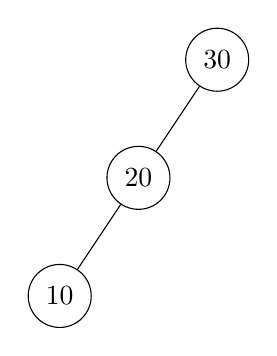
\begin{tikzpicture}[
                level distance=1.5cm,
                sibling distance=2cm,
                every node/.style={circle, draw, minimum size=0.8cm}
                ]
                % Unbalanced tree
                \node {30}
                child {node {20}
                    child {node {10}}
                    child[missing]
                }
                child[missing];
            \end{tikzpicture}
            \qquad
            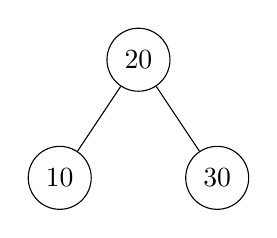
\begin{tikzpicture}[
                level distance=1.5cm,
                sibling distance=2cm,
                every node/.style={circle, draw, minimum size=0.8cm}
                ]
                % After right rotation
                \node {20}
                child {node {10}}
                child {node {30}};
            \end{tikzpicture}
        \end{latin}
        \caption{چرخش راست: گره ۲۰ به ریشه تبدیل می‌شود}
        \label{fig:right-rotation}
    \end{figure}
    
    \subsection{پیاده‌سازی}
    
    \begin{latin}
        \begin{minted}{python}
            from dataclasses import dataclass
            from typing import Optional
            
            
            @dataclass
            class AVLNode:
            key: int
            height: int = 1
            left: Optional['AVLNode'] = None
            right: Optional['AVLNode'] = None
            
            
            class AVLTree:
            """Self-balancing AVL tree implementation."""
            
            def height(self, node: Optional[AVLNode]) -> int:
            return node.height if node else 0
            
            def balance_factor(self, node: Optional[AVLNode]) -> int:
            return self.height(node.left) - self.height(node.right)
            
            def rotate_right(self, y: AVLNode) -> AVLNode:
            x = y.left
            T2 = x.right
            x.right = y
            y.left = T2
            y.height = 1 + max(self.height(y.left), self.height(y.right))
            x.height = 1 + max(self.height(x.left), self.height(x.right))
            return x
            
            def rotate_left(self, x: AVLNode) -> AVLNode:
            y = x.right
            T2 = y.left
            y.left = x
            x.right = T2
            x.height = 1 + max(self.height(x.left), self.height(x.right))
            y.height = 1 + max(self.height(y.left), self.height(y.right))
            return y
            
            def insert(self, node: Optional[AVLNode], key: int) -> AVLNode:
            """Insert a key and rebalance the tree."""
            if not node:
            return AVLNode(key)
            
            if key < node.key:
            node.left = self.insert(node.left, key)
            elif key > node.key:
            node.right = self.insert(node.right, key)
            else:
            return node  # Duplicate keys not allowed
            
            node.height = 1 + max(self.height(node.left),
            self.height(node.right))
            
            balance = self.balance_factor(node)
            
            # Left-Left case
            if balance > 1 and key < node.left.key:
            return self.rotate_right(node)
            # Right-Right case
            if balance < -1 and key > node.right.key:
            return self.rotate_left(node)
            # Left-Right case
            if balance > 1 and key > node.left.key:
            node.left = self.rotate_left(node.left)
            return self.rotate_right(node)
            # Right-Left case
            if balance < -1 and key < node.right.key:
            node.right = self.rotate_right(node.right)
            return self.rotate_left(node)
            
            return node
        \end{minted}
    \end{latin}
    \codecaption{درخت AVL با چرخش‌های خودکار}
    \label{code:avl}
    
    \section{درخت سرخ-سیاه}
    
    \subsection{تعریف}
    
    \begin{definition}[درخت سرخ-سیاه]
        یک درخت جستجوی دودویی که هر گره آن
        دارای یک \textbf{رنگ}\index{درخت سرخ-سیاه}
        (قرمز یا سیاه) است و پنج شرط زیر برقرار است:
        \begin{enumerate}
            \item هر گره یا قرمز است یا سیاه
            \item ریشه همواره سیاه است
            \item برگ‌های NIL سیاه هستند
            \item فرزندان یک گره قرمز، سیاه هستند
            \item تعداد گره‌های سیاه در مسیر از هر گره
            به برگ‌های NIL یکسان است
        \end{enumerate}
        \label{def:red-black}
    \end{definition}
    
    \begin{theorem}[ارتفاع درخت سرخ-سیاه]
        ارتفاع درخت سرخ-سیاه با $n$ کلید
        حداکثر $2\log_{2}(n+1)$ است.
        \label{thm:rb-height}
    \end{theorem}
    
    \subsection{عملیات درج}
    
    درج در درخت سرخ-سیاه شامل سه گام است:
    \begin{enumerate}
        \item درج مانند BST معمولی (گره جدید قرمز)
        \item رنگ‌آمیزی مجدد برای حفظ شرایط
        \item چرخش در صورت نیاز
    \end{enumerate}
    
    حالت‌های نقض شرط ۴ (پدر و عمو قرمز،
    عمو سیاه با ساختار مثلثی یا خطی).
    
    \begin{remark}
        درخت سرخ-سیاه در کتابخانه‌های استاندارد
        مانند \texttt{std::map} در C++ و
        \texttt{TreeMap} در جاوا استفاده می‌شود.
        دلیل انتخاب آن نسبت به AVL،
        تعداد کمتر چرخش‌ها در عملیات درج است.
        \label{rem:rb-vs-avl}
    \end{remark}
    
    \section{درخت B و B+}
    
    \subsection{انگیزه}
    
    برای داده‌های حجیم که در حافظه جا نمی‌شوند
    و روی دیسک\index{پایگاه داده} ذخیره می‌شوند،
    تعداد دسترسی‌های دیسک عامل تعیین‌کننده است.
    درخت B\index{درخت B} با افزایش ضریب انشعاب،
    ارتفاع را کاهش می‌دهد.
    
    \begin{definition}[درخت B از مرتبه $t$]
        \begin{itemize}
            \item هر گره (جز ریشه) حداقل $t-1$ کلید دارد
            \item هر گره حداکثر $2t-1$ کلید دارد
            \item هر گره با $k$ کلید، $k+1$ فرزند دارد
            \item تمام برگ‌ها در یک سطح هستند
        \end{itemize}
        \label{def:b-tree}
    \end{definition}
    
    ارتفاع درخت B با $n$ کلید:
    $h \leq \log_{t} \frac{n+1}{2}$
    
    \begin{figure}[h]
        \centering
        \begin{latin}
            \begin{tikzpicture}[
                level distance=1.8cm,
                sibling distance=3cm,
                bnode/.style={rectangle, draw=matindarkblue, fill=matinlightblue!30,
                    rounded corners, minimum width=4cm, minimum height=0.8cm}
                ]
                \node[bnode] {20 | 40 | 60}
                child {node[bnode] {5 | 10}}
                child {node[bnode] {25 | 30 | 35}}
                child {node[bnode] {45 | 50}}
                child {node[bnode] {70 | 80 | 90}};
            \end{tikzpicture}
        \end{latin}
        \caption{درخت B از مرتبه $t=3$ (درخت ۲-۳-۴)}
        \label{fig:b-tree}
    \end{figure}
    
    \subsection{درخت B+}
    
    \begin{definition}[درخت B+]
        مشابه درخت B، با دو تفاوت:
        \begin{enumerate}
            \item تمام کلیدها در برگ‌ها ذخیره می‌شوند
            (گره‌های داخلی فقط راهنما هستند)
            \item برگ‌ها به صورت لیست پیوندی
            به هم متصل شده‌اند
        \end{enumerate}
        \label{def:b-plus-tree}
    \end{definition}
    
    مزیت اصلی: پیمایش ترتیبی بسیار سریع
    و مناسب برای \textbf{پرس‌وجوهای بازه‌ای}
    در پایگاه داده.
    
    \section{درخت‌های تصادفی}
    
    \subsection{Treap}
    
    \begin{definition}[Treap]
        ترکیب \textbf{Tree} + \textbf{Heap}.
        هر گره یک کلید (طبق BST) و یک
        \textbf{اولویت تصادفی} (طبق Max-Heap) دارد.
        اولویت‌های تصادفی تضمین می‌کنند
        ارتفاع مورد انتظار $O(\log n)$ باشد.
        \label{def:treap}
    \end{definition}
    
    مزیت: پیاده‌سازی بسیار ساده‌تر از AVL
    و سرخ-سیاه. درج و حذف تنها با چرخش.
    
    \subsection{درخت جستجوی تصادفی}
    
    اگر عناصر را به ترتیب \textbf{تصادفی}
    در یک BST ساده درج کنیم،
    ارتفاع مورد انتظار $O(\log n)$ خواهد بود.
    این نتیجه از تحلیل Quick Sort می‌آید.
    
    \section{تحلیل پیچیدگی}
    
    \begin{table}[h]
        \centering
        \caption{پیچیدگی عملیات در درخت‌های متوازن}
        \label{tab:tree-complexity}
        \begin{tabular}{|c|c|c|c|c|}
            \hline
            \textbf{عملیات} & \textbf{AVL} & \textbf{سرخ-سیاه} & \textbf{B-Tree} & \textbf{Treap} \\
            \hline
            جستجو & $O(\log n)$ & $O(\log n)$ & $O(\log_{t} n)$ & $O(\log n)$* \\
            درج & $O(\log n)$ & $O(\log n)$ & $O(\log_{t} n)$ & $O(\log n)$* \\
            حذف & $O(\log n)$ & $O(\log n)$ & $O(\log_{t} n)$ & $O(\log n)$* \\
            چرخش در درج & $\leq 2$ & $\leq 2$ & تقسیم & $\leq 2$* \\
            چرخش در حذف & $O(\log n)$ & $\leq 3$ & ادغام & $O(\log n)$* \\
            \hline
        \end{tabular}
    \end{table}
    * مورد انتظار، نه بدترین حالت
    
    \section{تمرین‌ها}
    
    \begin{exercise}
        یک درخت AVL اولیه خالی را در نظر بگیرید.
        اعداد $10, 20, 30, 40, 50, 25$ را
        به ترتیب درج کنید و پس از هر درج،
        ساختار درخت را رسم کنید.
        \label{exc:avl-insert-sequence}
    \end{exercise}
    
    \begin{exercise}
        ثابت کنید ارتفاع درخت سرخ-سیاه
        با $n$ کلید داخلی حداکثر
        $2\log_{2}(n+1)$ است.
        \label{exc:rb-height-proof}
    \end{exercise}
    
    \begin{exercise}
        نشان دهید چرا درخت B برای ذخیره‌سازی
        روی دیسک مناسب‌تر از درخت دودویی است.
        زمان دسترسی به دیسک را $10$ میلی‌ثانیه
        و زمان پردازش در حافظه را $0.1$ میکروثانیه
        فرض کنید.
        \label{exc:b-tree-disk}
    \end{exercise}
    
    \begin{exercise}
        یک \lr{Treap} پیاده‌سازی کنید
        و ارتفاع آن را برای $n = 1000$ درج تصادفی
        به طور تجربی اندازه بگیرید.
        آزمایش را ۱۰۰ بار تکرار و میانگین را گزارش کنید.
        \label{exc:treap-experiment}
    \end{exercise}
    
    \begin{exercise}
        الگوریتم \textbf{ادغام} دو درخت AVL
        با پیچیدگی $O(\log n)$ را طراحی کنید.
        \label{exc:avl-merge}
    \end{exercise}
    
    %========================================
    % BIBLIOGRAPHY
    %========================================
    \begin{latin}
        \printbibliography[title={منابع و مراجع}]
    \end{latin}
    
    %========================================
    % INDEX
    %========================================
    \printindex
    
\end{document}